% \documentclass[table]{beamer}
\documentclass[table,handout]{beamer}
\setbeameroption{show notes}
% \setbeameroption{hide notes}
% \setbeameroption{show only notes}
\usepackage{varwidth}

\newif\ifhide
\newif\ifpost
\newif\ifhideclicker

% \hidetrue
% \hideclickertrue
% \posttrue

\newcommand{\whiteout}[1]{\textcolor{white}{#1}}
% \newcommand{\whiteoutbox}[1]{\fcolorbox{white}{white}{\parbox{\dimexpr \linewidth-2\fboxsep-2\fboxrule}{\whiteout{#1}}}}
% \newcommand{\notebox}[1]{\fcolorbox{blue}{white}{\parbox{\dimexpr \linewidth-2\fboxsep-2\fboxrule}{#1}}}
\newcommand{\whiteoutbox}[1]{\fcolorbox{white}{white}{\parbox{\linewidth}{\whiteout{#1}}}}
\newcommand{\notebox}[1]{\fcolorbox{blue}{white}{\parbox{\linewidth}{#1}}}
\newcommand{\blankbox}[1]{\phantom{\varwidth{\linewidth}\whiteoutbox{#1}\endvarwidth}}
\newcommand{\blank}[1]{\phantom{\varwidth{\linewidth}#1\endvarwidth}}

\ifhide%
    \newcommand{\hmask}[1]{\blank{#1}}%
\else%
    \newcommand{\hmask}[1]{#1}%
\fi

\ifhide%
    \newcommand{\wout}[1]{\whiteout{#1}}%
\else%
    \newcommand{\wout}[1]{#1}%
\fi

\ifhide%
    \newcommand{\hignore}[1]{}%
\else%
    \newcommand{\hignore}[1]{#1}%
\fi

\ifpost%
    \newcommand{\nopost}[1]{}%
\else%
    \newcommand{\nopost}[1]{#1}%
\fi

\ifhideclicker%
    \newcommand{\clickerslide}[1]{\stepcounter{clickerQuestionCounter}%
        \begin{frame}[t]
            \textcolor{blue}{Q \arabic{clickerQuestionCounter}:}
        \end{frame}}
\else%
    \newcommand{\clickerslide}[1]{#1}%
\fi

\ifhide%
    \newcommand{\hidebox}[1]{\blank{#1}}%
\else%
    \newcommand{\hidebox}[1]{\notebox{#1}}%
\fi

\ifhide%
    \newcommand{\wbox}[1]{\whiteoutbox{#1}}%
\else%
    \newcommand{\wbox}[1]{\notebox{#1}}%
\fi

\ifhide%
    \newcommand{\nbox}[1]{\blankbox{#1}}%
\else%
    \newcommand{\nbox}[1]{\notebox{#1}}%
\fi

\ifhideclicker%
    \newcommand{\clickeranswer}[1]{#1}%
\else%
    \ifhide%
        \newcommand{\clickeranswer}[1]{#1}%
    \else%
        \newcommand{\clickeranswer}[1]{\textbf{\textcolor{blue}{#1}}}%
    \fi
\fi

\usepackage{beamerthemesplit}
% \usetheme{boxes}
\usetheme{Malmoe}
\usecolortheme{seahorse}
% \usecolortheme{seagull}
\usepackage{ifthen}
\usepackage{xspace}
\usepackage{multirow}
\usepackage{multicol}
\usepackage{booktabs}
\usepackage{xcolor}
\usepackage{wasysym}
\usepackage{comment}
\usepackage{hyperref}
\hypersetup{pdfborder={0 0 0}, colorlinks=true, urlcolor=blue, linkcolor=blue, citecolor=blue}
\usepackage{changepage}
\usepackage[compatibility=false]{caption}
\captionsetup[figure]{font=scriptsize, labelformat=empty, textformat=simple, justification=centering, skip=2pt}
\usepackage{tikz}
\usetikzlibrary{trees,calc,backgrounds}

\usepackage[bibstyle=joaks-slides,maxcitenames=3,mincitenames=1,backend=biber]{biblatex}

\newrobustcmd*{\shortfullcite}{\AtNextCite{\renewbibmacro{title}{}\renewbibmacro{in:}{}\renewbibmacro{number}{}}\fullcite}

\newrobustcmd*{\footlessfullcite}{\AtNextCite{\renewbibmacro{title}{}\renewbibmacro{in:}{}}\footfullcite}

% Make all footnotes smaller
% \renewcommand{\footnotesize}{\scriptsize}

\definecolor{myGray}{gray}{0.9}
\colorlet{rowred}{red!30!white}

\setbeamertemplate{blocks}[rounded][shadow=true]

\setbeamercolor{defaultcolor}{bg=structure!30!normal text.bg,fg=black}
\setbeamercolor{block body}{bg=structure!30!normal text.bg,fg=black}
\setbeamercolor{block title}{bg=structure!50!normal text.bg,fg=black}

\newenvironment<>{varblock}[2][\textwidth]{%
  \setlength{\textwidth}{#1}
  \begin{actionenv}#3%
    \def\insertblocktitle{#2}%
    \par%
    \usebeamertemplate{block begin}}
  {\par%
    \usebeamertemplate{block end}%
  \end{actionenv}}

\newenvironment{displaybox}[1][\textwidth]
{
    \centerline\bgroup\hfill
    \begin{beamerboxesrounded}[lower=defaultcolor,shadow=true,width=#1]{}
}
{
    \end{beamerboxesrounded}\hfill\egroup
}

\newenvironment{onlinebox}[1][4cm]
{
    \newbox\mybox
    \newdimen\myboxht
    \setbox\mybox\hbox\bgroup%
        \begin{beamerboxesrounded}[lower=defaultcolor,shadow=true,width=#1]{}
    \centering
}
{
    \end{beamerboxesrounded}\egroup
    \myboxht\ht\mybox
    \raisebox{-0.25\myboxht}{\usebox\mybox}\hspace{2pt}
}

\newenvironment{mydescription}{
    \begin{description}
        \setlength{\leftskip}{-1.5cm}}
    {\end{description}}

\newenvironment{myitemize}{
    \begin{itemize}
        \setlength{\leftskip}{-.3cm}}
    {\end{itemize}}

% footnote without a marker
\newcommand\barefootnote[1]{%
  \begingroup
  \renewcommand\thefootnote{}\footnote{#1}%
  \addtocounter{footnote}{-1}%
  \endgroup
}

% define formatting for footer
\newcommand{\myfootline}{%
    {\it
    \insertshorttitle
    \hspace*{\fill} 
    \insertshortauthor, \insertshortinstitute
    % \ifx\insertsubtitle\@empty\else, \insertshortsubtitle\fi
    \hspace*{\fill}
    \insertframenumber/\inserttotalframenumber}}

% set up footer
\setbeamertemplate{footline}{%
    \usebeamerfont{structure}
    \begin{beamercolorbox}[wd=\paperwidth,ht=2.25ex,dp=1ex]{frametitle}%
        % \Tiny\hspace*{4mm}\myfootline\hspace{4mm}
        \tiny\hspace*{4mm}\myfootline\hspace{4mm}
    \end{beamercolorbox}}

% remove navigation bar
\beamertemplatenavigationsymbolsempty

\makeatletter
    \newenvironment{noheadline}{
        \setbeamertemplate{headline}[default]
        \def\beamer@entrycode{\vspace*{-\headheight}}
    }{}
\makeatother

\newcounter{clickerQuestionCounter}
\ifhideclicker%
\newenvironment{clickerquestion}
{ \stepcounter{clickerQuestionCounter}
  \begin{enumerate}[Q \arabic{clickerQuestionCounter}:]\color{white} }
{ \end{enumerate} }
\else%
\newenvironment{clickerquestion}
{ \stepcounter{clickerQuestionCounter}
  \begin{enumerate}[Q \arabic{clickerQuestionCounter}:] }
{ \end{enumerate} }
\fi

\ifhideclicker%
\newenvironment{clickeroptions}
{ \begin{enumerate}[\begingroup\color{white} 1)\endgroup]\color{white} }
{ \end{enumerate} }
\else%
\newenvironment{clickeroptions}
{ \begin{enumerate}[\begingroup\color{red} 1)\endgroup] }
{ \end{enumerate} }
\fi


\tikzstyle{centered} = [align=center, text centered, font=\sffamily\bfseries]
\tikzstyle{skip} = [centered, inner sep=0pt, fill]
\tikzstyle{empty} = [centered, inner sep=0pt]
\tikzstyle{inode} = [centered, circle, minimum width=4pt, fill=black, inner sep=0pt]
\tikzstyle{tnode} = [centered, circle, inner sep=1pt]
\tikzset{
  % edge styles
  level distance=10mm,
  mate/.style={edge from parent/.style={draw,distance=3pt}},
  mleft/.style={grow=left, level distance=10mm, edge from parent path={(\tikzparentnode.west)--(\tikzchildnode.east)}},
  mright/.style={grow=right, level distance=10mm, edge from parent path={(\tikzparentnode.east)--(\tikzchildnode.west)}},
  % node styles
  male/.style={rectangle,minimum size=4mm,fill=gray!80},
  female/.style={circle,minimum size=4mm,fill=gray!80},
  amale/.style={male,fill=red},
  afemale/.style={female,fill=red},
}

\newcommand{\highlight}[1]{\textcolor{violet}{\textit{\textbf{#1}}}}
\newcommand{\super}[1]{\ensuremath{^{\textrm{\sffamily #1}}}}
\newcommand{\sub}[1]{\ensuremath{_{\textrm{\sffamily #1}}}}
\newcommand{\dC}{\ensuremath{^\circ{\textrm{C}}}}
\newcommand{\tb}{\hspace{2em}}
\providecommand{\e}[1]{\ensuremath{\times 10^{#1}}}
\newcommand{\myHangIndent}{\hangindent=5mm}

\newcommand{\spp}[1]{\textit{#1}}

\newcommand\mybullet{\leavevmode%
\usebeamertemplate{itemize item}\hspace{.5em}}

\makeatletter
\newcommand*{\rom}[1]{\expandafter\@slowromancap\romannumeral #1@}
\makeatother

\newcommand{\blankslide}{{\setbeamercolor{background canvas}{bg=black}
\setbeamercolor{whitetext}{fg=white}
\begin{frame}<handout:0>[plain]
\end{frame}}}

\newcommand{\whiteslide}{
\begin{frame}<handout:0>[plain]
\end{frame}}

\newcommand{\f}[1]{\ensuremath{F_{#1}}}
\newcommand{\x}[1]{X\ensuremath{^{#1}}}
\newcommand{\y}[1]{Y\ensuremath{^{#1}}}

% Population growth macros
\newcommand{\popsize}[1]{\ensuremath{N_{#1}}}
\newcommand{\popgrowthratediscrete}[1]{\ensuremath{\lambda_{#1}}}
\newcommand{\popgrowthrate}[1]{\ensuremath{r_{#1}}}
\newcommand{\ptime}{\ensuremath{t}\xspace}

\tikzset{hide on/.code={\only<#1>{\color{white}}}}
\tikzset{
    invisible/.style={opacity=0},
    visible on/.style={alt={#1{}{invisible}}},
    alt/.code args={<#1>#2#3}{%
        \alt<#1>{\pgfkeysalso{#2}}{\pgfkeysalso{#3}}
        % \pgfkeysalso doesn't change the path
    },
}

\bibliography{../bib/references}
\author[J.\ Oaks]{
    %Jamie R.\ Oaks\inst{1}
    Jamie R.\ Oaks
}
\institute[BIOL 180]{
    \inst{}%
        BIOL 180: Introductory Biology
}



\title{Ecosystems I: Energy \& Nutrients}
% \date{\today}
\date{June 1, 2015}

% \setbeamertemplate{section in toc}[sections numbered]
% \setbeamertemplate{subsection in toc}[subsections numbered]

\begin{document}

\begin{noheadline}
\maketitle
\end{noheadline}

\nopost{
\begin{noheadline}
\begin{frame}[c]
    \vspace{-6mm}
    \begin{center} 
        \includegraphics[height=1.2\textheight]{../images/seating-chart-2.pdf}
    \end{center}
\end{frame}
\end{noheadline}
}

\clickerslide{
\begin{noheadline}
\begin{frame}
    \begin{adjustwidth}{-2em}{-1.5em}

        % \vspace{-3mm}

        \centerline{
            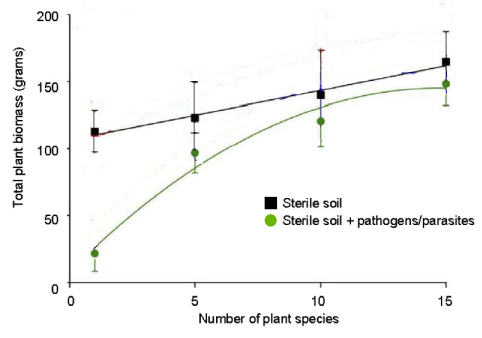
\includegraphics[height=0.65\textheight]{diversity-productivity-pathogen-clicker.png}}

        \vspace{-2mm}
        \begin{clickerquestion}
            \item What is the take-home message from comparing these graphs? 

            \begin{clickeroptions}
                \item \clickeranswer{Species-poor plots have low NPP due to
                        disease.}
                \item The sterilization process itself is responsible for the
                    differences observed.
                \item In disease-free environments, NPP does not change with
                    increasing species richness.
                \item In disease-free environments, NPP plateaus with
                    increasing species richness.
            \end{clickeroptions}
        \end{clickerquestion}
    \end{adjustwidth}
    \note[item]{What's the mechanism? More species, lower probability they will
        all be hit hard by disease (diseases are mostly species specific). In a
        monoculture = higher population density = higher transmission rates}
\end{frame}
\end{noheadline}
}

\begin{noheadline}
\begin{frame}
\frametitle{Today's issues:}
\vspace{5mm}
% \tableofcontents[subsectionstyle=hide]
\tableofcontents
\end{frame}
\end{noheadline}

\section{Global patterns of NPP}

\begin{frame}[t]
    \begin{adjustwidth}{-2em}{-1.5em}
        \vspace{-3mm}
        Patterns of net primary productivity I

        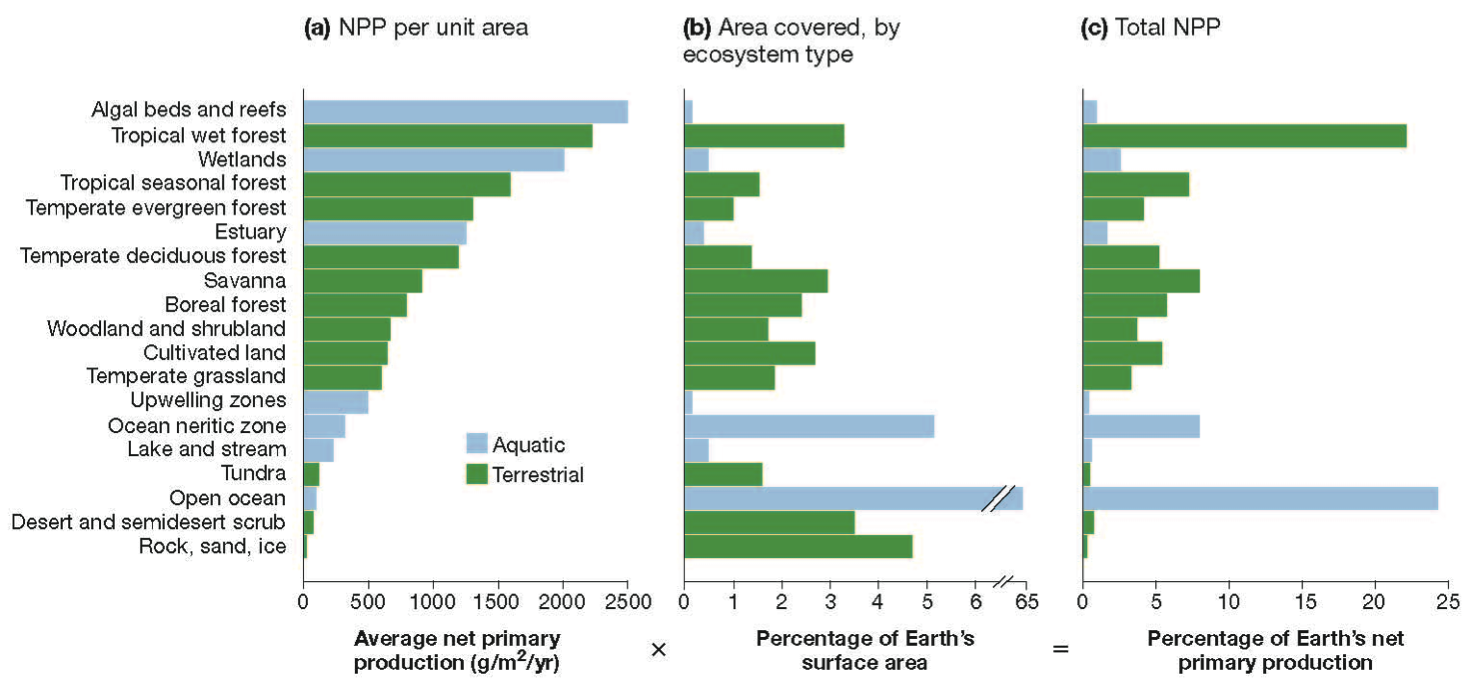
\includegraphics[width=\linewidth]{productivity-by-ecosystems.png}

        \vspace{-1mm}
        \begin{itemize}
            \small
            \item Where is NPP/km\super{2} relatively high? \cmask{\tiny
                    Tropical rainforests, algal beds/coral reefs, wetlands}

            \item Why is NPP/km\super{2} in the open ocean so low, if lots of
                light is available and the water is warm? \cmask{\tiny No
                    nutrients (non-living biomass sinks to bottom, where it's
                    very cold and there's no light)}

            \item Why does so much of the total NPP come from open ocean?
                \cmask{\tiny It's HUGE!}
        \end{itemize}

    \end{adjustwidth}
\end{frame}

\begin{frame}[t]
    \begin{adjustwidth}{-2em}{-1.5em}
        \vspace{-3mm}
        Patterns of net primary productivity II

        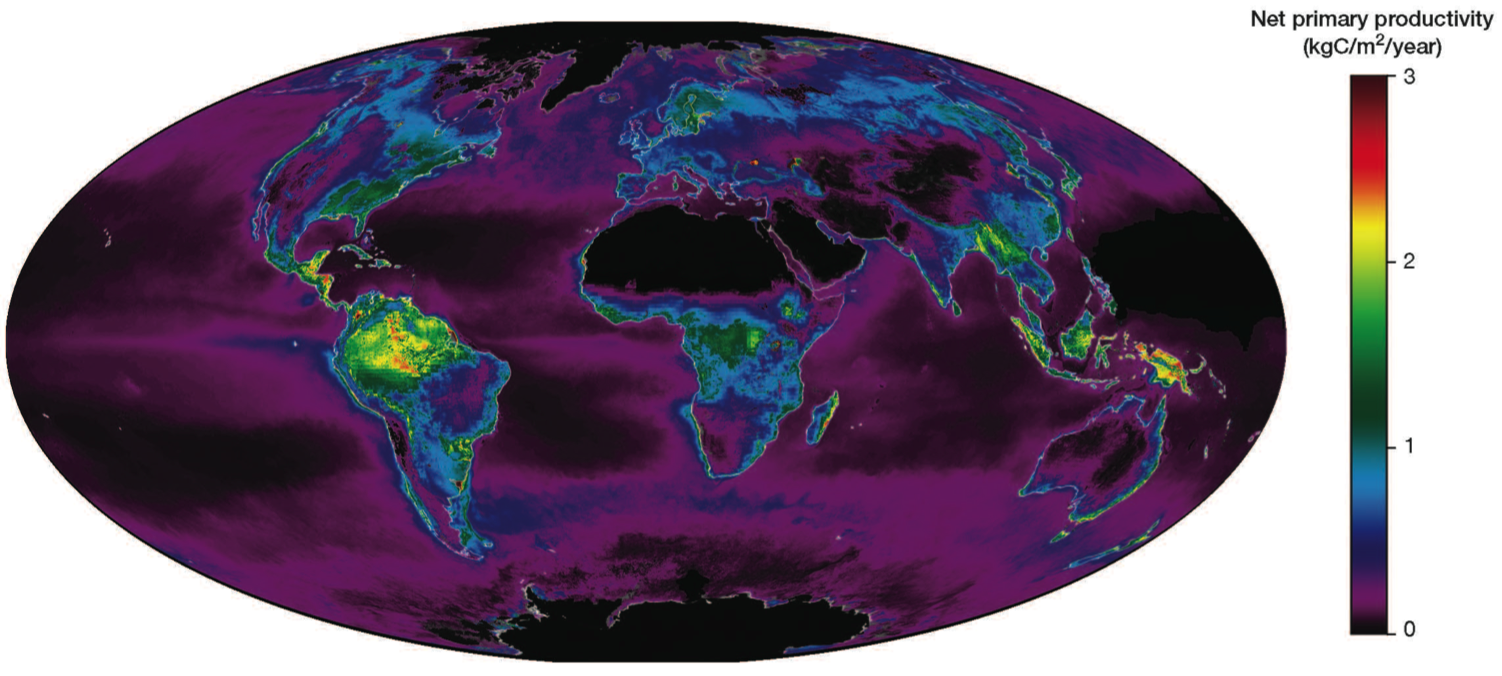
\includegraphics[width=\linewidth]{productivity-heat-map.png}

        \vspace{-2mm}
        \begin{itemize}
            \item Compare and contrast where terrestrial vs.\ marine
                productivity is high.

                \nbox{\tiny Terrestrial is highest near equator; marine is
                    highest along shorelines and high latitudes}

            \item Generally, what limits productivity in terrestrial habitats?

                \nbox{\tiny Temperature and water}

        \end{itemize}

    \end{adjustwidth}
\end{frame}

\clickerslide{
\begin{frame}
    \begin{clickerquestion}
        \item  Per m\super{2}, how does productivity compare in terrestrial
            vs.\ marine environments?

        \begin{clickeroptions}
            \item \clickeranswer{Terrestrial is much higher}
            \item Terrestrial is slightly higher
            \item About the same
            \item Marine is slightly higher
            \item Marine is much higher
        \end{clickeroptions}
    \end{clickerquestion}
\end{frame}
}

\clickerslide{
\begin{frame}
    \begin{clickerquestion}
        \item On a global scale, what is the most important limitation on
            productivity in marine habitats? 
 
        \begin{clickeroptions}
            \item \clickeranswer{Nutrients}
            \item Amount of incident radiation (sunlight)
            \item Water quality (pollution)
            \item Water temperature
        \end{clickeroptions}
    \end{clickerquestion}
\end{frame}
}

\begin{frame}[t]
    \begin{adjustwidth}{-2em}{-1.5em}

        % \vspace{-3mm}
        \begin{itemize}
            \item In the open ocean, what happens to nutrients available in
                organisms living at the surface?

                \nbox{\scriptsize Lots of sunlight at surface; primary
                    producers (PP) convert sunlight to biomass; uneaten PPs
                    sink to benthos when they die}

                \vspace{5mm}
            \item In the open ocean, why aren't nutrients recycled from the
                benthos?

                \nbox{\scriptsize It's cold and dark on the bottom; no primary
                    productivity. Nutrients can't get to the surface where the
                    PPs are}

                \vspace{5mm}
            \item Why are coastlines so productive?

                \nbox{\scriptsize When deep currents hit the continental shelf,
                    upwelling brings nutrients from the benthos to the
                    surface---available for PPs}
        \end{itemize}

    \end{adjustwidth}
\end{frame}

\section{How does energy flow through ecosystems?}

\begin{frame}[t]
    \begin{adjustwidth}{-2em}{-1.5em}
        \vspace{-3mm}
        How does energy flow through ecosystems?

        \uncover<2->{
        \vspace{2mm}
        Trophic levels in a Puget Sound food chain
        }

        \uncover<3->{
        \begin{table}%[htbp]
            \centering
            \begin{tabular}{ c c c }
                \multicolumn{1}{p{12mm}}{Trophic level} &
                \multicolumn{1}{c}{Feeding strategy} &
                \multicolumn{1}{c}{Grazing food chain} \\
                \hline
                5 & 4\degree consumer & Orcas \\[2ex]
                4 & 3\degree consumer & Salmon \\[2ex]
                3 & 2\degree consumer & Herring \\[2ex]
                2 & 1\degree consumer & Copepods \\[2ex]
                1 & Autotroph (PP) & Algae \& bacteria \\ 
            \end{tabular}
        \end{table}
        }

        \uncover<4->{
        \begin{itemize}
            \item What about orcas that eat seals (seals eat salmon)?
                \nbox{\scriptsize Many consumers eat at multiple trophic
                    levels}

            \item How would a Puget Sound food WEB be different?

                \nbox{\tiny Rather than showing one pathway of energy
                flow across trophic levels (like the food chain above), it
                would show ALL the possible pathways; it would be a network of
                all energy transfered among all species in the community}
        \end{itemize}
        }
    \end{adjustwidth}
    \note[item]{What about orcas that eat seals (seals eat salmon)}
    \note[item]{Many consumers eat at multiple trophic levels}
    \note[item]{How would a Puget Sound food web be different?}
\end{frame}


\begin{frame}[t]
    \begin{adjustwidth}{-2em}{-1.5em}
        \vspace{-3mm}
        Energy (NPP) data from Hubbard Brook Experimental Forest

        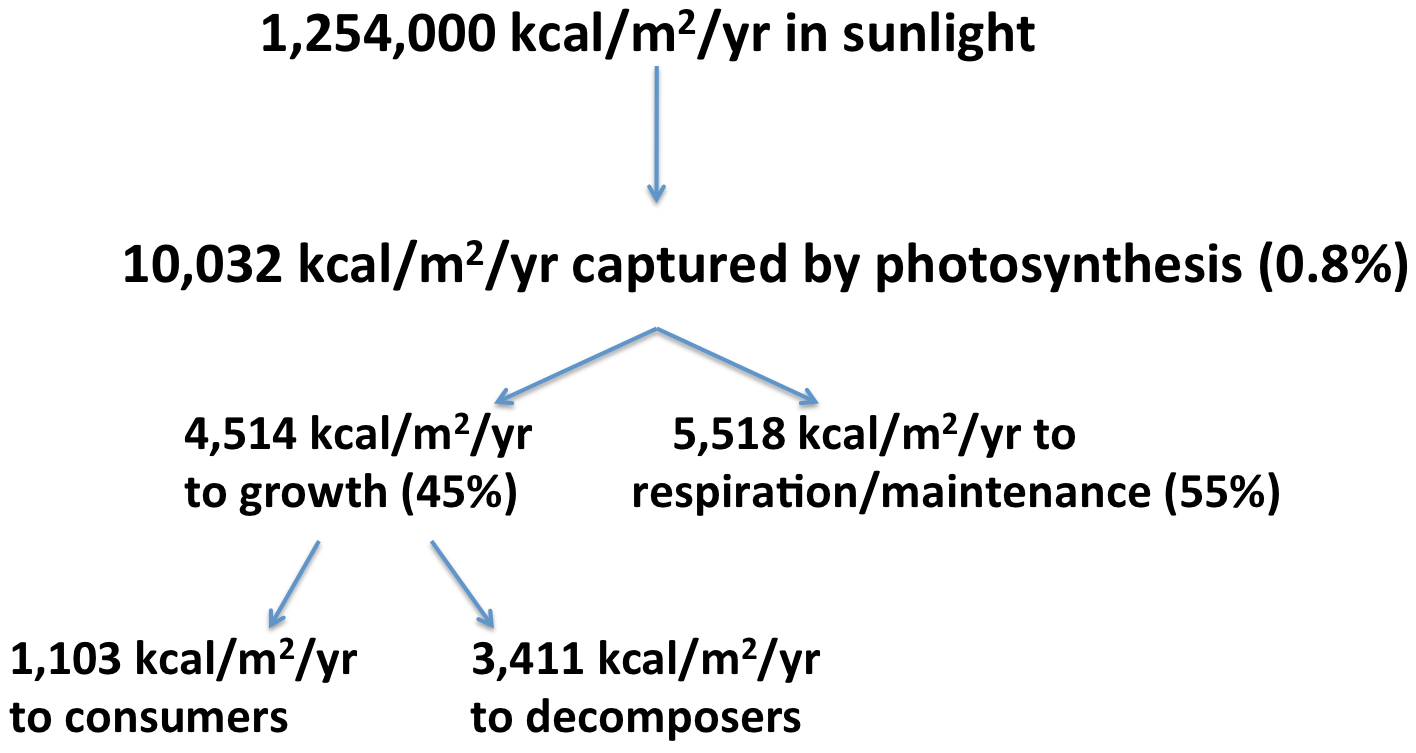
\includegraphics[width=\linewidth]{energy-transfer-cascade.png}

        In this ecosystem, what percentage of NPP gets eaten as living tissue?
        
        \nbox{\tiny $(1103/4514)100 = 24\%$}

    \end{adjustwidth}
    \note[item]{What number is GPP? What number is NPP?}
\end{frame}

\begin{frame}[t]
    \begin{adjustwidth}{-2em}{-1.5em}
        \vspace{-3mm}
        Efficiency of energy transfer across trophic levels at Hubbard Brook

        \vspace{-1mm}
        \begin{center}
        \begin{tikzpicture}[>=latex]%,xscale=0.3,yscale=0.3]
        
            % \tikzstyle{state} = [draw, fill=structure!20!, rectangle,
            \tikzstyle{state} = [fill=white, rectangle,
                minimum height=2em,
                minimum width=4em,
                node distance=4em,
                font={\sffamily}]
            \tikzstyle{stateEdgePortion} = [black,ultra thick];
            \tikzstyle{stateEdge} = [stateEdgePortion,->];
            \tikzstyle{edgeLabel} = [pos=0.5, text centered, font={\sffamily\small}];
        
            % Reservoirs
            \node[visible on=<6->, state, name=c3] {\textcolor{blue}{3
                    g/m\super{2}/yr of tertiary consumer biomass (10\%
                    efficiency)}};
            \node[visible on=<5->, state, name=c2, below of=c3]
            {\textcolor{blue}{30 g/m\super{2}/yr of secondary consumer biomass
                    (15\% efficiency)}};
            \node[visible on=<4->, state, name=c1, below of=c2]
            {\textcolor{blue}{200 g/m\super{2}/yr of primary consumer biomass
                    (20\% efficiency)}};
            \node[visible on=<3->, state, name=pp, below of=c1]
            {\textcolor{blue}{1000 g/m\super{2}/yr of primary producer biomass
                    (NPP)}};
            \node[visible on=<2->, state, name=sun, below of=pp]
            {\textcolor{blue}{$\approx$1\% of sunlight to GPP}};
        
            % Connect States via edges
            \begin{uncoverenv}<3->
            \draw ($(sun.north)
                    + (0,0)
                $) 
                edge[stateEdge] node[edgeLabel,
                    % xshift=-3em
                ]{} 
                ($(pp.south)
                    + (0,0)
                $); 
            \end{uncoverenv}
            \begin{uncoverenv}<4->
            \draw ($(pp.north)
                    + (0,0)
                $) 
                edge[stateEdge] node[edgeLabel,
                    % xshift=-3em
                ]{} 
                ($(c1.south)
                    + (0,0)
                $); 
            \end{uncoverenv}
            \begin{uncoverenv}<5->
            \draw ($(c1.north)
                    + (0,0)
                $) 
                edge[stateEdge] node[edgeLabel,
                    % xshift=-3em
                ]{} 
                ($(c2.south)
                    + (0,0)
                $); 
            \end{uncoverenv}
            \begin{uncoverenv}<6->
            \draw ($(c2.north)
                    + (0,0)
                $) 
                edge[stateEdge] node[edgeLabel,
                    % xshift=-3em
                ]{} 
                ($(c3.south)
                    + (0,0)
                $); 
            \end{uncoverenv}
        \end{tikzpicture}
        \end{center}

        \uncover<7->{
        \vspace{-3mm}
        {\small NOTE: Productivity pyramids represent maximum possible energy
            transfer.  What does this mean? \cmask{\tiny Assumes all new
                biomass at each level is eaten by next level}}
        }

    \end{adjustwidth}
\end{frame}

\begin{frame}[t]
    \begin{adjustwidth}{-2em}{-1.5em}
        \begin{itemize}
            \item Why is so much energy lost at each transfer?

                \nbox{Some of what is eaten is not assimilated (lost in feces).
                    A large proportion that is assimilated is used for cellular
                    respiration (digestion, immune defense, repair/maintenance,
                    movement, heat, etc.); NOT biomass.}

                \vspace{4mm}
            \item Which is more efficient as a primary consumer, a fish or a
                cow? Why?

                \nbox{Fish---it does not use energy to maintain body
                    temperature (ectothermic)}

                \vspace{8mm}
            \item Clams and mussels eat detritus as well as small primary
                producers and consumers. Would you consider them an efficient
                consumer? Why or why not?

                \nbox{Yes---they are consuming from both food chains (i.e.,
                    living (grazing) and non-living (decomposing)). Also, they
                    are ectothermic and move very little.}

        \end{itemize}

    \end{adjustwidth}
\end{frame}

\clickerslide{
\begin{frame}
    \begin{clickerquestion}
        \item At Hubbard Brook, why does the \highlight{efficiency} of energy
            transfer decline as you go up each trophic level? 
 
        \begin{clickeroptions}
            \item There are fewer predators than prey.
            \item All tertiary consumers are endotherms and lose a great deal
                of energy as heat.
            \item Species diversity is not as high at the upper trophic levels.
            \item \clickeranswer{In order to find food, consumers at higher
                    trophic levels have to move around a lot more than
                    lower-level consumers.}
        \end{clickeroptions}
    \end{clickerquestion}
\end{frame}
}

\clickerslide{
\begin{frame}
    \begin{clickerquestion}
        \item On a per-gram basis, large mammals have lower metabolic rates
            than smaller mammals. Based on this observation, which mammals
            should convert primary production to biomass more efficiently? 

        \begin{clickeroptions}
            \item \clickeranswer{Large mammals}
            \item Small mammals
            \item No difference, because the comparison was done on a per-gram
                basis
        \end{clickeroptions}
    \end{clickerquestion}
\end{frame}
}

\section{How do nutrients flow through ecosystems?}

\begin{frame}[t]
    \begin{adjustwidth}{-2em}{-1.5em}
        How do nutrients flow through ecosystems? (biogeochemical cycles)

        \begin{itemize}[<+->]
            \item E.g., Nitrogen cycle, water cycle, carbon cycle, etc.

                \vspace{8mm}
            \item Atoms move through ecosystems, among organisms in food webs,
                and between organisms and the abiotic environment. (They are
                recycled)

                \vspace{8mm}
            \item Humans are altering most biogeochemical cycles in
                massive ways.

                \begin{itemize}
                    \item E.g., the nitrogen cycle (We are doubling natural N
                        inputs!).
                \end{itemize}
        \end{itemize}

    \end{adjustwidth}
\end{frame}

\begin{frame}[t]
    \begin{adjustwidth}{-2em}{-1.5em}
        The Dead Zone in the Gulf of Mexico

        \begin{enumerate}
            \item Lots of nitrates (from ammonia-based fertilizer) run
                off farm fields into the Mississippi River and into
                the Gulf.

            \item In response, \wout{huge increase in primary production by
                    photosynthetic algae and bacteria = eutrophication}

            \vspace{6mm}
            \item \wout{Primary producers die (short-lived; rapid turnover)}

            \vspace{6mm}
            \item \wout{\small Huge increase in primary decomposers (eating
                    all the dead algae/bacteria)}

            \vspace{6mm}
            \item \wout{Oxygen depleted by decomposers}

            \vspace{6mm}
            \item \wout{Fish and other oxygen-dependent species die}
        \end{enumerate}

        \vspace{4mm}
        \uncover<2->{This happens in Hood Canal, and many other places, too}

    \end{adjustwidth}
\end{frame}

\end{document}

\clickerslide{
\begin{frame}
    \begin{clickerquestion}
        \item 
        \begin{clickeroptions}
            \item 
            \item 
            \item 
            \item 
        \end{clickeroptions}
    \end{clickerquestion}
\end{frame}
}

\clickerpost{
{
\usebackgroundtemplate{\includegraphics[page=17,width=\paperwidth]{./24-Radiation-extinction.pdf}}
\begin{frame}[t,plain]
    \begin{adjustwidth}{-2em}{-1.5em}
        \cmask{Answer: 3}
    \end{adjustwidth}
\end{frame}
}
}

